\subsection{Original implementation}

The code of the previously proposed implementation is shown in Listing~\ref{lst:naive_mm}.
Since in the section above we benchmark the compiled code on matrices of size multiple of 8 and in any case ensured to be like that due to the \texttt{-DALIGN} flag, for consistency purposes we will also include that flag in every proposed tests. 

Also for continuity purposes we will show results from \textbf{ICC}, omitting the one from ICX and GCC (since they do not provide any observation  that was not already discussed).

The integrated OpenMP implementation for the baseline algorithm is detailed in Listing~\ref{lst:orig_openmp}.

\begin{lstlisting}[style=CStyle, caption={Original algorithm with OpenMP directives: the parametrization is managed at runtime.}, label={lst:orig_openmp}]
int n_threads;
omp_sched_t runtime_schedule_type;
int block_size;

void multiply_matrices(int n,
    m_type (*restrict A)[n], m_type (*restrict B)[n], m_type (*restrict C)[n])
{
    (*@\textcolor{red}{omp\_set\_schedule(runtime\_schedule\_type, block\_size);} @*)
    (*@\textcolor{red}{omp\_set\_num\_threads(n\_threads);} @*)
    
    (*@\textcolor{red}{\#pragma omp parallel for shared(A, B, C, n) schedule(runtime)}   @*)   
    for (int i = 0; i < n; ++i)
        for (int k = 0; k < n; k++)
            for (int j = 0; j < n; ++j)
                C[i][j] += A[i][k] * B[k][j];
}
\end{lstlisting}

\subsubsection{Concurrency}
Now that we have a general overview of the problem, we can start with the empirical investigation.
First, we can propose an \emph{educated guess} about the best number of threads we can concurrently use.

As reported in Table~\ref{tab:cpu_specs}, the studied hardware integrate 8 single-threaded core, and 8 2-way simultaneous-multithreaded cores; we can hence suppose the sweet-spot will in be in the range 16-24 (more than that will produce more threads than cores, wasting computational time by executing context-switches).

The empirical results are shown in Figure~\ref{fig:orig_tune_t}, and they confirm our hypothesis choosing \textbf{\texttt{T=24}} as the best choice.

\begin{figure}[H]
    \centering
    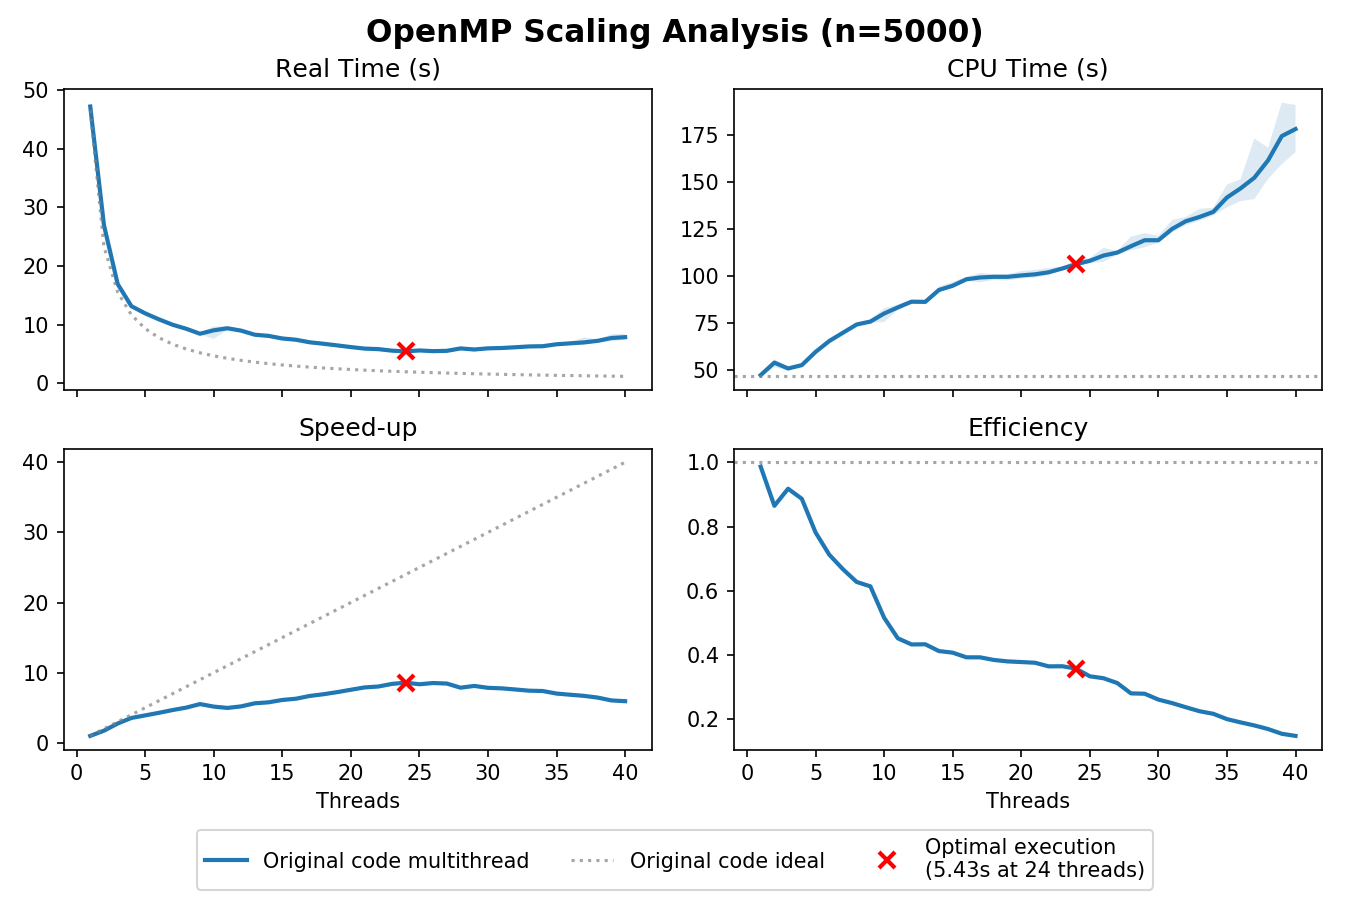
\includegraphics[width=\textwidth]{Images/orig_t_tuning.png}
    \caption{Hyper-parameter tuning of the naive algorithm on $T$, evaluated on matrix \texttt{n=5000} }
    \label{fig:orig_tune_t}
\end{figure}

Comparing these results with the equivalent sequential baseline (which computes a matrix of size \texttt{n=5000} in \textbf{6.5 seconds}), we evaluated the multi-threaded execution using the \emph{Speed-up} and \emph{Efficiency} metrics (introduced in Section~\ref{subsubsec:metrics}). 

The results show a performance degrated so much that it cannot only be caused by multi-threading overhead operations: investigating the compiler's optimization reports clearly shows that introducing the OpenMP directives forces the compiler to avoid the aggressive loop transformations that it typically applies under the \texttt{-O3} flag. 

Once assessed this problem, further hyper-parameter tuning of the naive algorithm is futile. Consequently, we will abandon this implementation and transition to exploring only our custom BLAS-like implementation.



